\chapter{Introduction}

\introquote{
    \textsc{Caliban} \\[-5pt]
    You taught me language, and my profit on ’t \\[-5pt]
    Is I know how to curse. The red plague rid you  \\[-5pt]
    For learning me your language!\\
}{
    William Shakespeare, \textit{The Tempest} (I.ii.362-364)
}

\introquote{
    \textbf{[Prompt]} Q: How many eyes does a horse have? \\[-5pt]
    \textbf{[GPT-3]} A: 4. It has two eyes on the outside and two eyes on the 
        inside.
}{
    GPT-3 \citep{brown2020}, responding to a prompt by \cite{shane2020}
}

\addvspace{6\bigskipamount}

\startglyph Somewhere out of
the inky-black terminals and  unseeable valleys of high-dimensional
loss-surfaces, an unexpectedly expressive capacity to generate natural
language has emerged in contemporary models of machine learning.
In particular, deep learning-based language models have dramatically improved
the overall quality of computer generated text, opening the doors to many
exciting applications like creative writing tools
\citep{huggingface2019,samuel2019,seabrook2019} and interactive fiction
\citep{robertson2019}.  While these new natural language generation (NLG)
methods are quite powerful, they are in practice very difficult to control or
constrain. This is unfortunate as it limits responsible application to domains
with high fault tolerance, like the those mentioned above and other,
essentially low stakes, human guided creative exploration tools. It is unclear
if such tools are ready for real deployments in crisis informatics
\citep{starbird2013} or medicine \citep{gatt2009}.

This thesis is focused on a particular text-to-text generation problem,
automatic summarization, where the goal is to map a large input text to a much
shorter summary text, and the research presented aims to both understand and
tame these machine learning d{\ae}mons, hopefully paving the way for more
reliable text-to-text~generation algorithms.  Somewhat against the prevailing
trends, we eschew end-to-end training of an abstractive summarization model,
and instead breakdown the text summarizaion problem into its consituent tasks.
At a high level, we divide these tasks into two categories: \textit{content
selection}, or ``what to say'' and \textit{content realization}, or ``how to
say it'' \citep{mckeown1985}.  Within these categories we propose models and
learning algorithms for the following problems:
    
\begin{itemize}
  \item Content Selection
  \begin{itemize}
    \item Salience Estimation with Deep Learning Content Selection Models
    \item Salience Estimation with Structured Content Selection Models
  \end{itemize}
  \item Content Realization
  \begin{itemize}
    \item Data Augmentation and Self-Training for Faithful Neural NLG Models
    \item Meaning Representation Linearization Strategies for Content Planning
          and Controllable Neural NLG Models
  \end{itemize}
\end{itemize}

The first part, content selection, explores various issues around salience
estimation, that is, predicting the importance of an arbitrary unit of text
given some surrounding context (e.g., the larger document that contains that
text or a user query). In particular, we experiment with a variety of popular
and novel deep learning models for salience estimation, and design several
ablation exeriments to gain some insight into which input signals are most
important for making predictions. Understanding these signals is critical for
designing reliable summarization models. 

We then consider a more difficult problem of estimating salience in a large
document stream, and propose two alternative approaches using classical
machine learning techniques from unsupervised clustering and structured
prediction. These models incorporate salience estimates into larger text
extraction algorithms that also consider redundancy and previous extraction
decisions.
    
In part two, content realization, we assume content selection has already been
performed and focus on methods for faithful generation, i.e., ensuring that
output text utterances respect the semantics of the input content. Since they
can generate very fluent and natural text, deep learning-based NLG~models are
a popular approach to this problem. However, they often omit, misconstrue, or
otherwise generate text that is not semantically correct given the input
content. In this section, we develop a data augmentation and self-training
technique to mitigate this problem. Additionally, we propose a training method
for making deep learning-based NLG models capable of following a content plan,
allowing for more control over the output utterance generated by the model.
Finally, under a stress test evaluation protocol, we demonstrate some
empirical limits on several neural NLG models' ability to encode and properly
realized a content plan.
 
It is important to note that the approaches in part two are implemented for
solving \textit{task-oriented dialogue generation} \citep{mairesse2010}, where
the problem is one of modeling the response of a dialogue agent interacting
with a human user. The input in this setting is a formal meaning
representation of both the communicative goal that the dialogue agent is
trying to achieve and the content that is to be realized. While this is
technically a data-to-text and not a text-to-text generation problem, the aims
of faithful and controllable generation are relevant to both problem classes.
With data-to-text generation, however, we get an explicit representation of
meaning that makes it easier to measure progress in model faithfulness and
control. We therefore consider task-oriented dialogue generation as an
idealized form of text-to-text generation, where a content selection module
has mapped input text units to a discrete meaning representation for realizing
the content.  Possible methods of transferring these approaches to the
text-to-text regime will be discussed in \autoref{ch:conclusion}.


\section{Problems in Text-to-Text Generation}
  
Amongst the natural language processsing (NLP) research community, machine
learning, and especially deep learning, has become the \latin{de facto}
epistemological and methodological framework  for solving text-to-text
generation problems.  One need only to obtain a large collection of
input-output texts, and under this paradigm, the details of the particular
generation task can be abstracted away. It is sufficient to re-pose the
generation problem as a one of optimization, for which a general purpose
neural network model can be trained such that it minimizes the relevant loss
function, and in so doing, learns a mapping from the input text to the output
text \citep{sutskever2014,bahdanau2015,rush2015,nallapati2016,see2017}. 

That is to say, the deep learning framework de-emphasizes possessing a
``theory of the problem'' to be solved, and prefers instead a hands off
approach: the theory of the problem is implicit in the dataset, so let the
neural network, whose inductive bias is very different from that of the human
researcher, learn directly from the data the representations that are most
useful to its satisfaction of the optimization criteria.\footnote{One could
reasonably argue that language models have been evolving in the direction of
fewer inductive priors: ngram-models assert that the last few words are most
important; recurrent neural networks, the current word and as much as what can
be stuffed into a single memory vector; recurrent neural networks with
attention, the current word and any previous memory vector; and transformers,
random access memory to any input time step.} The logical extension of this
central dogma is that the best data is more data \citep{halevy2009}.  

And indeed that is precisely what has happened. Large language model
pre-training, where a language model, typically using a transformer
architecture \citep{vaswani2017}, is trained in a self-supervised way on
web-scale text, has dramatically expanded the quality of natural language
utterances that can be generated by a computational model
\citep{radford2019,brown2020}, while also capturing the attention of the
popular press \citep{simonite2019,vincent2019}. In the NLP research community,
pretrained sequence-to-sequence models, the family of deep learning model most
commonly used for text-to-text generation, like PEGASUS \citep{zhang2019}, T5
\citep{raffel2020}, or BART \citep{lewis2020}, have led to impressive gains in
the fluency and coherence of modestly-sized paragraphs, as well as automatic
task metrics like \bleu~\citep{papineni2002} and \rouge~\citep{lin2004}.

There are downsides to this approach however. By learning only from
surface level forms, it is possible for the models to appear like they contain
knowledge, but in reality, they are only modeling the probability of word sequences \citep{bender2020}. This can cause them to hallucinate information not present in the input or imply propositions contrary to what was given 
\citep{wiseman2017,kryscinski2019,maynez2020,kryscinski2020}.
Without an understanding of pragmatics, they cannot know how an argument
or chain of propositions
holds together, only that they are statistically likely.
Moreover, they will learn many implicit and harmful biases of the
society that produced the corpora they are trained on, including but 
not limited to negative stereotypical word associations \citep{bolukbasi2016,nissim2020} and outright 
hate speech \citep{lee2016}.

With all of that in mind, we would like this thesis to emphasize the theory
of the problems we are trying to solve. While we do not abandon
 machine learning
and deep learning, we instead show how they may be used parsimoniously to solve
the actual problems at hand and not simply learn the dataset. Where we 
do use machine learning models, we try to design experiments which 
reveal which signals 
relevant to the actual problem are being used to make predictions, and 
to establish some empirical limitations on their ability to represent 
the input data and perform successfully. 
%We posit that this is the 
%both a resposibility and boon of research on these models, as it can be used
%beyond the problem at hand.
 
In order to learn the theory of the problem, as we have been calling it, 
we must have some problems. We now describe some of the central problems
of summarization and text-to-text generation that we are interested in solving.
%% v%One of the logical conclusions of this framework is that more 
%% data is 
%% 
%% 
%% 
%% ~\\~\\
%% 
%% Under this paradigm, one
%% can ignore the details of the particular text-to-text problem at hand, and 
%% instead collect a large collection of input and output texts, and propose a general purpose 
%% solution 
%% as has allowed
%%  to abstract away the details of the summarization task, and 
%% build large neural network models with the capacity to map a document 
%% text to  
%% In particular, deep learning-based
%% language model pretraining on web-scale data \citep{} has both captured
%% the public imagination, but also led to real improvements 
%% 
%% 
%% \Deeplearning~models in 
%% particular have shown themselves to be both versatile and empirically 
%% successful solutions. However, the inner workings of such models are often 
%% opaque and difficult to 
%% control or understand in practice. In this thesis, we offer modeling 
%% methodologies to establish control or understanding in a variety of  
%% \machinelearning-based models of summarization. 
%% %At a high level, the 
%% %first two chapters focus on \contentselection.
%% %The last chapter focuses on \surfacerealization, that is, generating text
%% %from an idealized representation of the content selection stage. 
%%   
%% %  In this section, we will briefly introduce the tasks and problems that will 
%% %  ground the experiments and analyses of this work. More formal definitions
%% %  can be found in the individual chapters. 
%%   %It is for this reason that we focus on extractive summarization in this work.
%%   %\Automaticsummarization~as it is studied in the 
%%   %\naturallanguageprocessing~literature typically dichotomizes summarization
%%   %approaches into either \extractive~versus \abstractive~methods \cite{something}. 
%%   %In the former case, a summary is constructed by essentially copying and 
%%   %pasting the input utterances to obtain a summary; in the latter case, the 
%%   %summary content is generated from scratch, synthesizing the input content in
%%   %some manner to produce the summary. In practice, systems are often composed of
%%   %a mixture of extractive and abstractive techniques, e.g., using sentence 
%%   %compression on top of extraction. We study the extractive task since it allows
%%   %us to focus on the salience estimation task directly, while not having to
%%   %implement an abstractive generation component (which is typically more
%%   %computation and memory intensive than, and more difficult to evaluate). 
%%   %
In most summarization tasks, we are generally interested in a text's
\textit{\salience}, that is to say, the general importance or relevance of a
given text unit with respect to its context. \Salience~is usually the primary
dimension of the input data that we wish to measure or predict for
determining summary content.  

In \autoref{ch:dlsum}, we study \salienceestimation~in
the \emph{sentence extractive, single document summarization task}, where the
goal is to classify which sentences in an input document should be included in
an extract summary.  In this case, the input document is the context, and the
units of text for which we are estimating salience are the document sentences.
An extractive summary is a subset of sentences that have maximum salience
while sastifing a length budget constraint, typically in the summary word or
byte length. While the constrained subset selection problem is interesting and
has been studied previously \citep{goldstein1998,mcdonald2007,lin2010}, we
focus on modeling the salience estimation task specifically. 
 
We study a variety of popular and novel deep learning architectures for
implementing the salience prediction task. Our key contributions here are not only a 
model architecture, but also our systematic study of the combination of sentence
and context (i.e. document) level encoders as well as the manipulation of the
input documents to ablate which surface features are available to a given
model. Through these input data ablations, we can gain a better understanding
of how the salience prediction mechanism is working.
 
But what about more difficult summarization tasks? In \autoref{ch:mlsum}, we
study salience estimation for \emph{query focused, streaming, sentence
extractive summarization}. In this task, we add a search query and time as
additional elements to the summarization problem. As input we are given a
time-ordered stream of news articles and a query, typically a notable
real-world event, e.g., \texttt{``hurricane sandy''}. Our objective is to
extract sentences that are relevant to the query event while minimally
redundant to previously extracted sentences. Unlike the previous problem, the
salience of a given sentence is not constant but monotonically decreases as time
progresses. Due to the large volume of input texts, in attempting to 
model the salience of a sentence we must now also model the 
redundancy between sentences and previous extraction decisions to perform
competently.
      
We incorporate a salience estimation model into two possible approaches to
extracting query-relevant summary sentences from the news stream.  The first
method uses the salience estimates to bias an affinity propagation clustering
algorithm \citep{dueck2009} to identify exemplar sentences which we extract for the
summary.  The clustering algorithm must trade off representativeness versus
the salience of individual sentences when selecting exemplars, i.e. an
exemplar must be a good representative of its cluster but also be important
under the salience estimator.  This approach works in hourly batches,
predicting the salience of sentences, clustering them, and then adding the
exemplars to a rolling update summary. The salience estimates also adaptively
control the number of clusters produced, allowing the model to adapt the
number of updates to fit the volume of salient sentences found in the stream. 

The first method has several draw backs. The summary selection is not done
to optimize the final summary evaluation measure and the predictions of salience
are static and cannot take into account previous decisions the summarizer
has made. Additionally, the use of clustering means that there will always be 
some latency between when important information is known and when we can
extract it for the summary. In domains like crisis informatics, minimizing
these delays are critical \citep{starbird2013}.

To address these limitations, we recast stream summarization as a sequential
decision-making problem \citep{littman1996}, where we learn a policy for
extracting a sentence based on its estimated salience as well as its relation
to previously extracted sentences.  The sequential decision-making view opens
our model up to exposure bias as the learned policy will suffer from a
train-test distribution mismatch if our reference policies are overly
optimistic or pessimistic.  To mitigate this, we employ a learning-to-search
style training regime \citep{chang2015} to train a policy to make locally optimal
decisions when following either a noisy learned policy or an oracle reference
policy.  The result is a fully online summarization model whose local
decisions positively correlate with good overall summary evaluation measures.
Additionally, because the model is greedy, it does not suffer as much from the
negative effects of latency as the clustering model does.
      

In our experiments with single-document extractive summarization, we found
that neural models heavily exploited position-based heurstics (i.e., did the
sentence occur in the lead paragraph) to determine sentence salience, which
arguably does not capture the essence of the summarization problem. In our
work on stream summarization, we show that with careful feature and model
design, we can capture salience beyond such heuristics.  In particular, we
show that content, location, and redundancy features can be used to predict
salience in this more challenging scenario.
      


In \autoref{ch:nlg}, we move to problems of content realization, after the
content selection process has been performed.  Here we focus on the related
goals of \term{faithful}~and~\term{controllable}~generation using neural NLG
models. A neural NLG model is faithful if it can generate utterances that are
semantically correct with respect to the information extracted in the content
selection stage.  One of the central tensions in a neural NLG model is that
between the encoder, which creates a representation of the input, and the
decoder, which is functionally a language model conditioned on the encoder
representation.  The decoder language model must simultaneously place high
probability on output word sequences that are likely given the training
corpus, but also prefer output word sequences that are correlated with the
encoder representation of the input sequence. This conflict can lead to hallucinations as the language model
may occasionally put more probability mass on a sequence of words that is
frequently observed in the training data, but not necessarily licensed by 
a particular
input.

We hypothesize that this failure mode happens in part because the decoder,
by predicting next word continuations, is both
implicitly planning the layout of the utterance but also trying to satisfy the
constraints given by the input, and that alleviating the decoder language
model of the planning task may improve the faithfulness.  We propose
developing controllable neural NLG models, i.e. models that can
follow an explicit plan determining  the surface realization order of the
intended utterance.  Controllable models learn to represent the layout
of the intended utterance implicitly in their encoder, and thus the decoder
language model has less flexibility in selecting the next words, which can
lower the chances of hallucinating text and improve the overall faithfulness
of the generation model.

We also believe that controllable generation has additional benefits beyond
increased faithfulness. For one, it will enable more integration of neural NLG
models into large NLG pipelines, \citep{castroferreira2019}.
Controllable generation at the level of shallow phrase chunk ordering like
we are proposing may also lead to 
implimentations of cognitively
plausbile discourse ordering theories like Centering Theory \citep{grosz1995} or Accessibility Theory \citep{ariel2001}, which place constraints on the discourse ordering of entities.




%~\\~\\
%
%
%
%A neural NLG models will generate semantically correct utterances but 
%the decoder language model implicitly controls the surface realization order by
%generating the utterance one word at a time. We hypothesize that 
%
%
%  
%
%
%
%We attempt to resolve this tension,
%
%
%~\\ ~\\
% By alleviating the planning that the
%decoder language model in a neural NLG model must perform, we can also improve
%the faithfulness of the resulting model.
%
% To that end,
%we develop
%training the procedure that results in a controllable neural NLG model
%
%~\\~\\
%      %a reframing of the evaluation of \naturallanguagegeneration~from fluency and
%      %to semantic correctness 
%Controllable generation models represent a subset of faithful generation
%models.  
      
Evaluating the faithfulness of a language generation model for open-world
summary generation tasks is non-trivial \citep{kryscinski2020,maynez2020}. In
order to simplify things, we study faithful and controllable generation in the
context of task-oriented dialogue generation, where given an explicit
representation of a dialogue agent's belief state and goals, we must generate
an appropriate natural language utterance. Because the input is an explicit,
formalized representation of the meaning of the intended utterance, manual and
even automatic checking of the faithfulness of an utterance/meaning
representation pair becomes much simpler. Since the concerns of faithful and
controllable generation are still incredibly important to generating
summaries, we consider the explicit meaning representations as an idealized
version of summarization system's content selection stage.  Faithfulness is
critical for any real summarization application; the reader has to be able to
trust that content is correct or it is functionally useless. Controllable
generation will further increase reliability and faithfulness, while
also allowing the tailoring of the summary to focus on particular
user needs, for example targeting generation to focus on a particular set of
entities. 
      
      
      %In \taskorienteddialoggeneration, the dialog agent
      %has a communicative goal that it is trying to achieve. Crucially,
      %the input to the agent is an explicit representation of the meaning 
      %of intended utterance.
      %
      %
      %In \autoref{gen}, we move to the \datatotext~problem of 
      %\emph{\taskorienteddialoggeneration}, where given an explicit representation
      %of a dialog agent's belief state and goals, we must generate an appropiate
      %natural language utterance. In \taskorienteddialoggeneration, the dialog agent
      %usually has a goal that they need to achieve. For example, a dialog agent may
      %want to book a reserveration at a restaurant but inorder to do that, it 
      %needs to ask a user for a range of possible times that are acceptable to
      %place the reservation. In this case, input to the dialog generation 
      %component would be a representation describing a \texttt{request information} dialog act, with the desired missing information explicitly represented,\texttt{reservation time range}.
      %
      %When deep learning models are used to generate text in scenarios like these,
      %they are usually effective at generating fluent and natural text \cite{}.
      %However, without careful treatment, the frequently generate utterances
      %that do not accurate reflect the input meaning representation. In the
      %case above for example, they might accidentally request the  location 
      %instead of the time. 
      
      
For our contribution to faithful generation, we propose a novel data
augmentation method for sequence-to-sequence models.  We observe that a
popular sequence-to-sequence NLG model trained on a task-oriented dialogue
generation dataset produces fluent and natural utterances that are
unfortunately frequently semantically incorrect with respect to the input
meaning representation.  We then present evidence that the reason for these
errors are spurious correlations between the inputs and outputs in the
training data.  We also note that by injecting random noise into the
unfaithful NLG model we can cause it behave in an uncontrolled but useful
manner: it generates utterances that are not faithful to the input but do not
exhibit the spurious correlations or exhibit them to a lesser degree.  We
generate a synthetic corpus of these utterances, and then use another semantic
parsing model to given them correct meaning representations.  Remarkably,
sequence-to-sequence models trained on the union of original training data and
the synthetically generated training examples exhibit increased faithfulness
without hurting their fluency. We also find that in the union dataset, 
the problematic spurious correlations are diminished.

While this data augmentaiton method helps reduce semantic errors, it leaves the surface
realization of utterances up to the decoder language model. 
Our second contribution to neural NLG models is an alignment training method
that reliably produces controllable language generators. Our method works
by aligning the indvidual components of a meaning representation to their
reference utterances on the training set. Given this alignment, we then
map a meaning representation into a linear sequence of tokens, such that 
the order of the individual components corresponds to the realization order
in the training reference. Training an arbitrary sequence-to-sequence model
to map this linearized meaning representation to its reference utterance induces 
the ability to control the model at test time. I.e., we can use a planning
model to propose an ordering of the meaning representation's sub-components,
and the controllable sequence-to-sequence model will attempt to 
realize them in that order.
To achieve a different ordering, one need only permute the input sequence.

In our experiments, we also evaluate how well models are able to follow 
adversarially generated plans that do not have human, English language ordering
preferences and show that models struggle to realize utterances correctly in
this setting. We finally propose another data augmentation scheme to 
generate constituent phrase data that gives explicit examples of how
phrases can be composed into larger units and how that systematically
changes the meaning representation. We find that this additional data
improves the robustness of the control behavior on these more difficult to
follow plans.


%We also investigate an encoder input transformation, applicable to arbitrary \sequencetosequence~models, that reliably results in a controllable generation 
%model. 
 
%
%
%
%
%~\\~\\
%meaning representation 
%
%do not exhibit those spurious 
%
%
%
%Under our proposed
%protocol, we train an initial sequence-to-sequence NLG model to map meaning
%representations to natural language utterances. 
%This model 
%
%We also train a meaning representation
%parser model to map utterances back to meaning representations using the same
%data.  We then use a noise-injection scheme to perturb the NLG model sample
%a  diverse and semantically divergent. Because of the noise-injection, 
%the NLG model produces examples that break the spurious correlations in 
%training set. 
%
%that uses an
%        unfaithful NLG model and an model 
%      to generate novel and semantically diverse utterance/meaning representation 
%      pairs that can be used as additional training data. 
%
%Sequence-to-sequence
%      models trained on the union of original training data and the synthetically
%      generated training examples exhibit increased faithfulness.
      
      % to remove spurious correlations from the 
      %training data and obtain a 
      %neural \naturallanguagegeneration~model with reduced semantic errors.
      
     
      
      %
      %it occurs in)
      %
      %We start in the single document extractive summarization case, 
      %where the task is 
      %to predict a subset of an article's sentence to include in a summary.
      %We explore several popular neural architectures for performing this 
      %task and systemaically evaluate them under different noisy input ablations.
      %These ablations allow us to isolate different features of the input.
      %
      %
      %In the second chapter, we explore two classical machine learning models
      %applied to the harder problem of query focused extractive stream summarization. 
      %In this setting we propose two models, one that 
      
  \section{Contributions}
  
  We now briefly summarize the contributions of this thesis described
  in the previous sections.
  
  %This thesis  makes the following contributions to NLG.
  %In the areas of text-to-text generation,
  
  \begin{enumerate}
          \item We propose a systematic evaluation of deep learning models
              for extractive single document summarizations (\autoref{}). 
              Our evaluation on several popular neural architectures shows 
              that:
              \begin{itemize}
                  \item Position features, even when not explicitly represented
                      in the model architecture are a dominant feature
                      exploited by the model.
                  \item Content features exist across a variet of word classes
                      but are not as strong of a signal as position.
                  \item Word embedding averaging is about as effective as 
                      recurrent or convolutional sentence encoders 
              \end{itemize}
          \item Additionally, in the task of query focused streaming news 
              summarization, we propose two models for providing 
              extractive update summaries. (\autoref{})
              \begin{itemize}
  
                  \item The first method processes the stream in  batches. 
                      It uses a regression model
                      to estimate the salience of individual 
                      sentences, and a biased clustering algorithm to select
                      the most representative and salient outputs.
                  \item The second method processes the stream in a fully
                      online manner. A linear model makes extraction
                      decisions, and we experiment with a learning-to-search
                      algorithm for training. 
              \end{itemize}
      \end{enumerate}
  
      In the area of data-to-text generation, we make the following 
      contributions to faithful and controllable generation of 
      text from a meaning representation. 
      \begin{enumerate}
          \item We propose a noise injection and self-training method
              for obtaining a faithful NLG model.
          \item We propose an encoder input linearization called alignment
              training which  yields an NLG model with surface level
              realisation ordering control.
      \end{enumerate}
  
  
  Finally, in chapter \autoref{conc} we conclude with a discussion of the 
  limitations and future 
  directions this work might take. In particular, we focus on how 
  faithful generation might be applied to summarization or \machinetranslation
  where an explicit representation of the content meaning is not available. 
  



%%%    
%%%    
%%%    
%%%   



%%%    In the remainder of this chapter we briefly give some historical context
%%%    for the field \naturallanguagegeneration. 
%%%    We then introduce the main contributions of the thesis in more detail
%%%    before diving into main the chapters on content selection and surface 
%%%    realization. 
%%%    
%%%    
%%%    
%%%    %can be thought of 
%%%    %as bipartite modules consisting of encoder, which learns to represent and decoder are quite capable
%%%    %of generating fluent text, but there is a fundamental tension between the
%%%    %
%%%    %\deeplearning~based conditional language models produce output text utterances
%%%    %that do not semantic
%%%    %
%%%    %
%%%    %
%%%    %
%%%    %
%%%    %In the interest of developing more reliable \machinelearning~models for 
%%%    %\texttotext~generation problems, particularly 
%%%    %text summarization where a large input text is mapped to a smaller output
%%%    %summary text, we eschew the 
%%%    %
%%%    %
%%%    %\texttotext~generation, this papepr 
%%%    %
%%%    %
%%%    %In this work we study several popular models, and propose some of our own,
%%%    %for both \texttotext~and \datatotext~generation problems, with the 
%%%    %aim of designing experiments to give insight into what signals present in
%%%    %the data are actually being used for making predictions, and where possible,
%%%    %provide mechanisms or training strategies for control and systematic behavior. 
%%%    %
%%%    %
%%%    %
%%%    %Since  `
%%%    %
%%%    %
%%%    %
%%%    %
%%%    %In this work we explore two modalities of NLG, \texttotext and \datatotext 
%%%    %generation.
%%%    %
%%%    %
%%%    %In this work, we 
%%%    %explore two applied \naturallanguagegeneration settings, text-to-text and data-to-text
%%%    %
%%%    %
%%%    %
%%%    %Natural language generation (NLG) is a subfield of artificial 
%%%    %intelligence and computational linguistics broadly interested in algorithms
%%%    %for generating natural language text and speech \citep{reiter2000building},
%%%    %where the natural languages constitute those naturally arising in 
%%%    %human-to-human communication and contrasted with formal languages like LISP, Prolog, or Python \citep{}.
%%%    %This thesis makes contributions to two areas of NLG, 
%%%    %text summarization and data-to-text generation, using machine learning
%%%    %models, and especially deep learning or deep neural network models. 
%%%    %
%%%    %Machine learning models on natural language data
%%%    %can be inscrutable and unpredictable d{\ae}mons, especially as their complexity
%%%    %grows. One of the main goals of this work is to understand how
%%%    %such models make their decisions, what their limitations are, and how they
%%%    %may be used in a more controlled manner. Before further 
%%%    %developing our contributions, we begin with some historical context.
%%%    %
%%%    \begin{figure}
%%%        \centering
%%%    
%%%    
%%%        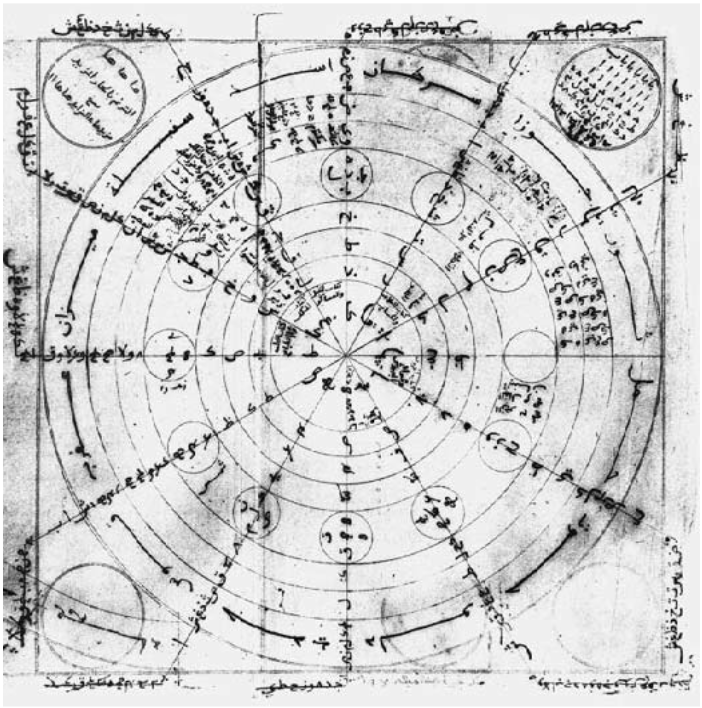
\includegraphics[width=0.49\textwidth]{ch1/images/zairja.png}
%%%        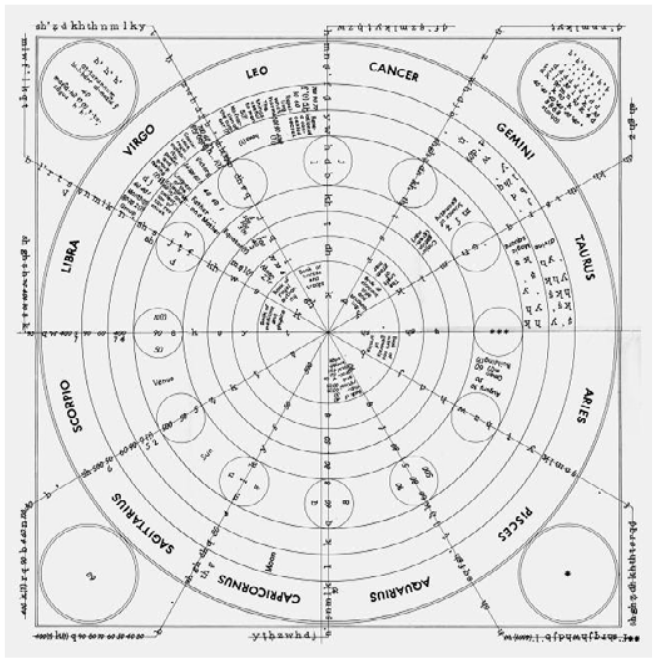
\includegraphics[width=0.49\textwidth]{ch1/images/zairjatl.png}
%%%        
%%%        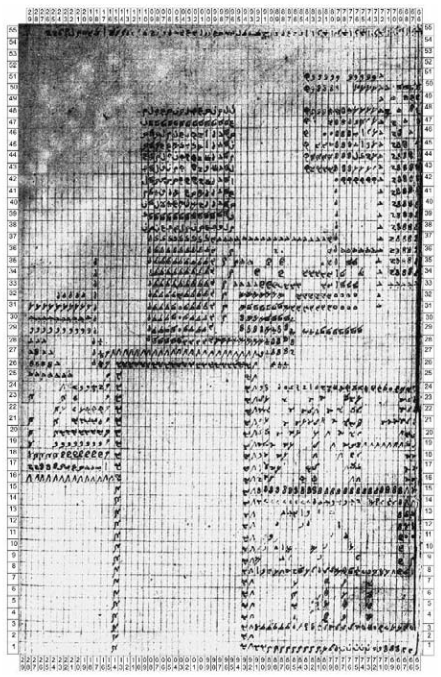
\includegraphics[width=0.6\textwidth,angle=90]{ch1/images/zairjaback.png}
%%%    
%%%        \caption{A zairja from a 15\textsuperscript{th} century Turkish manuscript of the \textit{Muqaddimah} \citep{link2010variantology}
%%%            (top left), its transliteration from the English translation
%%%        of \cite{rosenthal1958muqaddimah} (top right), and its lookup table (bottom).}
%%%        \label{fig:zairja}
%%%    \end{figure}
%%%    
%%%    
%%%    {\color{red} Note to Kathy: the history of nlg sections are rough and I need to change them to reflect a new way of organizing the paper that I settled on so you can probably just skip ahead to section 1.4 on page 12.}
%%%    
%%%    \section{A Brief History of NLG (antiquity-1950)}
%%%    
%%%    The desire to build machines
%%%    that manipulate human languages is an old one. 
%%%    One early account of a language generation algorithm 
%%%    comes from 
%%%    14\textsuperscript{th} century historian 
%%%    `Abd ar-Rahm\={a}n ibn Khald\={u}n (1332 -- 1406), who
%%%    writes in the \textit{Muqaddimah} (1377) of a circular prognostication 
%%%    and divining tool  used by Sufi mystics called a \textit{z\={a}'irjah}.\footnote{Franz Rosenthal in his English translation of the  \textit{Muqaddimah} suggests the name is derived from 
%%%    the Persian words z\={a}'icha meaning ``horoscope'' or  ``astronomical table''
%%%     and d\={a}'ira meaning ``circle.''}
%%%     Its practice is
%%%    ``a branch of the science of letter magic, practiced among the authorities on letter magic, is the technique of finding out answers from questions by means of connections existing between the letters of the expressions used in the question.'' 
%%%    Ibn Khald\={u}n points to an earlier treatise by the Sufi scholar 
%%%    Abu al-Abbas as-Sabti
%%%    (1129 -- 1204) of Marrakesh as a source of instructions for the device's use
%%%    \citep{rosenthal1958muqaddimah}, suggesting the practice is at least as
%%%    old at the 12\textsuperscript{th} century.
%%%    
%%%    The \textit{z\={a}'irjah} itself consists of a series of concentric circles divided into 12 
%%%    sections by six chords. The various segments of the diagram are annotated with 
%%%    letters and numerals. Additionally, the \textit{z\={a}'irjah}  is accompanied by a lookup table mapping
%%%    letters to numbers. See \autoref{fig:zairja} for an example. According to painstaking reconstructions done by \citep{link2010variantology},
%%%    a ``key poem'' was used to pose a question to the \textit{z\={a}'irjah} and serve as a 
%%%    mnemonic device/mapping of letters to entries in the lookup table. 
%%%    A combination of rules and astronomical observations (the 12\textsuperscript{th} century equivalent of a random seed)
%%%    were then applied to the key poem to read off series of characters from
%%%    the \textit{z\={a}'irjah}. The operator
%%%    would then interpret those letters into an answer.  
%%%    ``The fact that only consonants are written down in Semitic languages permits the meaningful interpretation of many random permutations of symbols,'' \citep{link2010variantology} suggesting that cherry-picking outputs and over-ascribing 
%%%    intelligence to a language generation algorithm are as old as the practice of
%%%     NLG itself.
%%%    
%%%    \begin{figure}
%%%        \centering
%%%        
\includegraphics[width=0.48\textwidth]{ch1/images/llull.png}
%%%        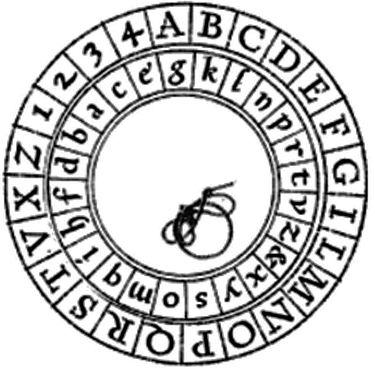
\includegraphics[width=0.48\textwidth]{ch1/images/cipher.JPG}
%%%        \caption{(Left) A \textit{volvelle} from  Llull's \textit{Ars Magnus} 
%%%        and (right) Alberti's cipher disk.}
%%%        \label{fig:llull}
%%%    \end{figure}
%%%    
%%%    \begin{figure}
%%%        \centering
%%%        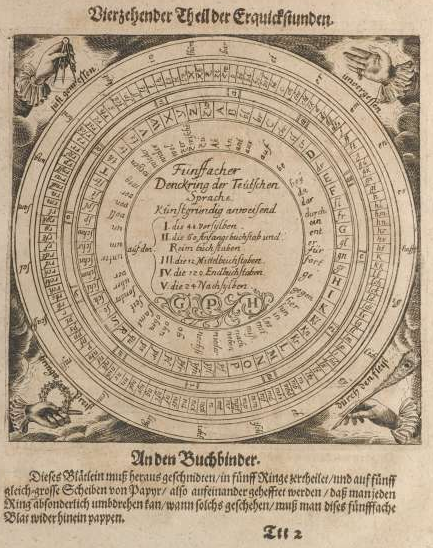
\includegraphics[width=0.98\textwidth]{ch1/images/baroqe.png}
%%%    
%%%        \caption{An illustration of the German word generator, \textit{F{\"u}nffacher Denckring der Teutschen Sprache}.}
%%%        \label{fig:denckring}
%%%    \end{figure}
%%%    
%%%    
%%%    
%%%    In a secondary account from a manuscript found at the library of Rabat, 
%%%    Morroco, it is written that a skeptical ibn Khald\={u}n asked of the device
%%%    how old it was: 
%%%    ``[Is the] z\={a}'irjah [a] recent or [an] ancient science?'' 
%%%    and received the answer: ``The  Holy  Spirit  will  depart,  
%%%    its  secret  having
%%%    been brought forth / To Idr\={\i}s, and through it, 
%%%    he ascended the highest summit,'' drawing a connection to the sage
%%%    Idr\={\i}s who is one of the eldest
%%%    ancestors in the Quranic tradition \citep{rosenthal1958muqaddimah,link2010variantology}.
%%%    
%%%    
%%%    
%%%    The teachings of Arabic mystics, including the practice of \textit{z\={a}'irjah}, as well 
%%%    as the Kabbalistic tradition embodied in the \textit{Sefer Yetzirah}
%%%    are known to have strongly influenced the 
%%%    Majorcan Christian mystic, Ramon Llull (1232-1315) \citep{kahn1980,sepllull,link2010variantology}.
%%%    %is known to have Arabic tradition  
%%%    %\textit{Z\={a}'irjah} are known to have influenced and similar practices from the Kabbalistic tradition 
%%%    %(the Sefer Yetzirah specifically) are known to have influenced the 
%%%    Llull, who is regarded as an early philosopher of combinatorics, logic, and 
%%%    computation \citep{sepllull,bonner2007art,knuth2013art}, developed 
%%%    a computational system based on moveable concetric circles made of paper
%%%    and connected by string. The workings of these \textit{volvelle}\footnote{The
%%%        name \textit{volvelle} 
%%%    comes from the Latin, literally ``to turn''} are described in his master work,
%%%    \textit{Ars Magna} (1305). According to his system, concepts were assigned
%%%    letters which were manipulated to generate new knowledge and he claimed 
%%%    could be used to determine the truth of any proposition 
%%%    \citep{Crupi2019VolvellesOK}. Llull's work is also thought to have influenced 
%%%    the polyalphabetic substitution cipher developed by Leon Battista Alberti 
%%%    (1404 -- 1472) (see \autoref{fig:llull}), the same core cryptographic technology used 
%%%    in the Enigma machine  \citep{kahn1980}.
%%%    
%%%    
%%%     \begin{figure}
%%%        \center
%%%        \noindent
%%%        {%
%%%            \setlength{\fboxsep}{0pt}%
%%%            \setlength{\fboxrule}{1pt}%
%%%            \fbox{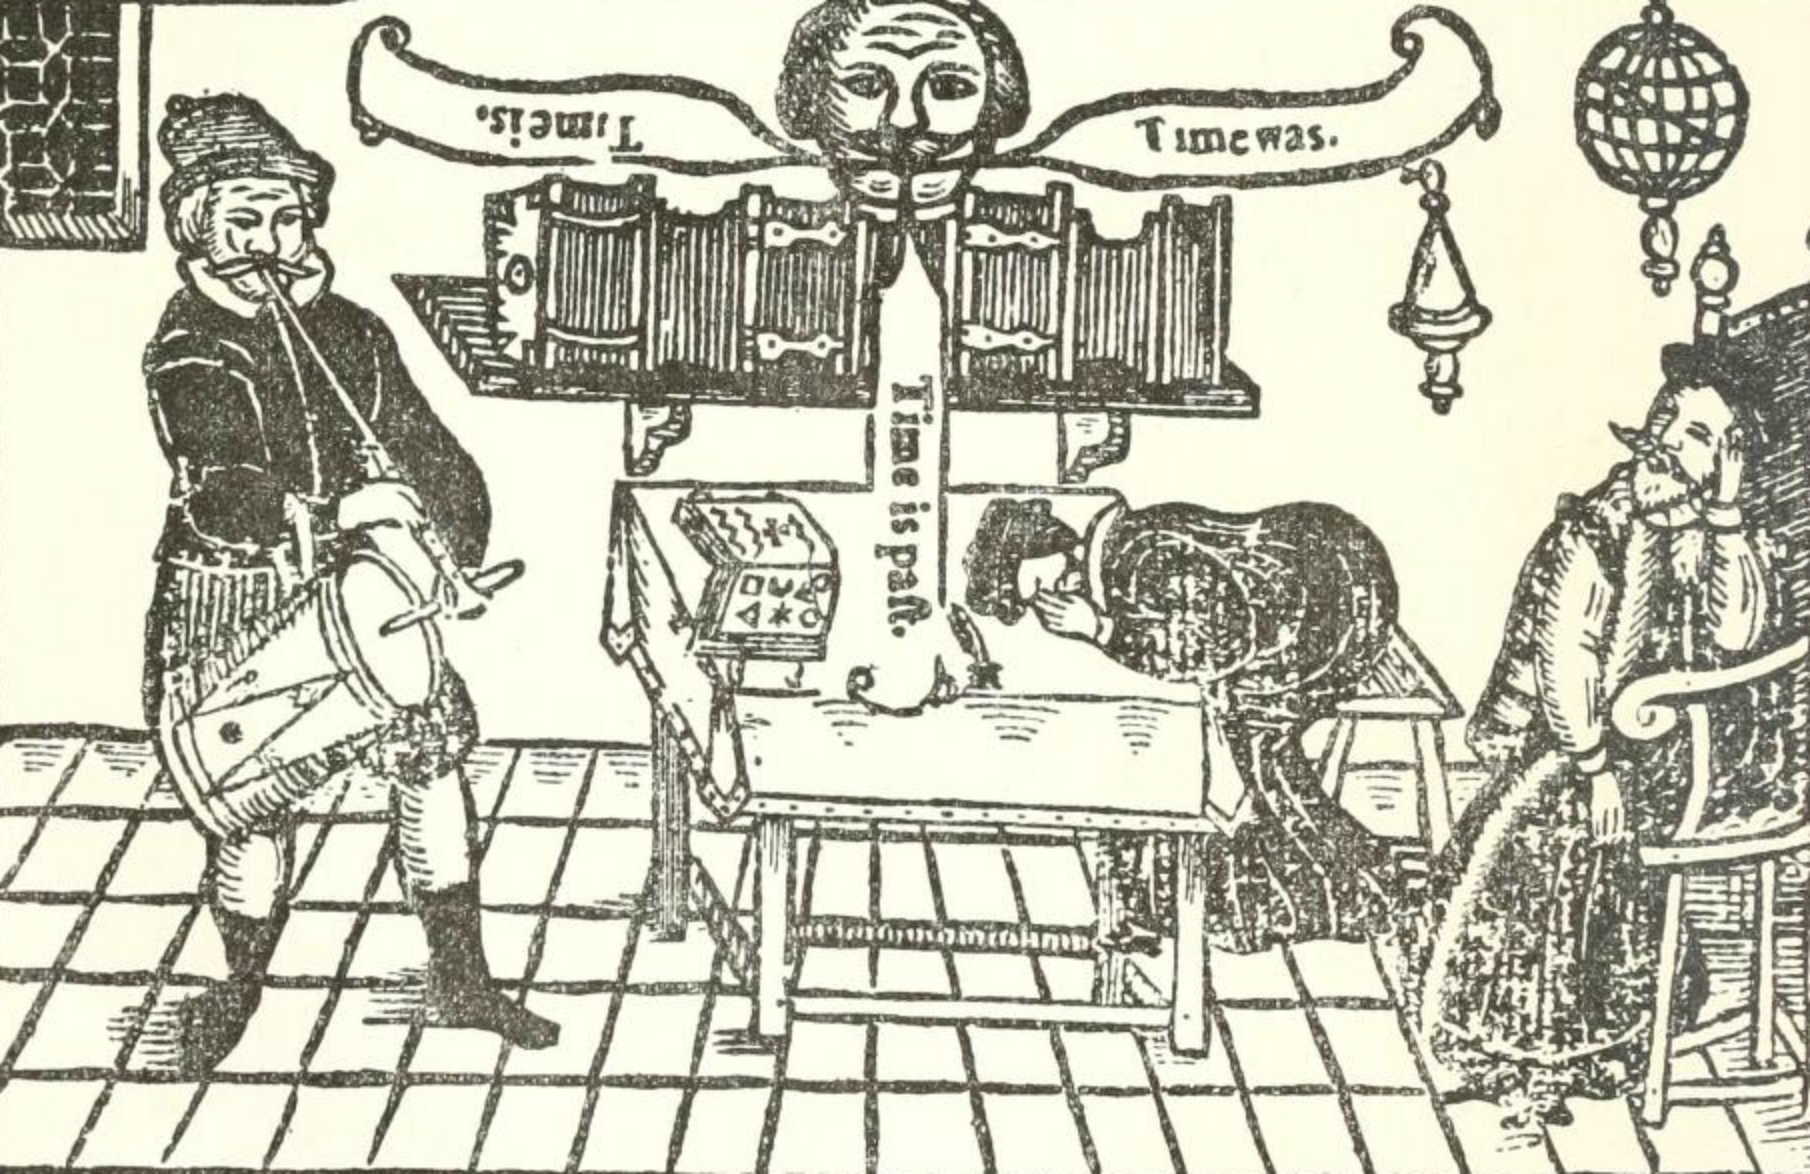
\includegraphics[width=0.7\textwidth]{brazen_head.png}}
%%%    }
%%%    \caption{A 1630 woodcut depicting Roger Bacon's talking bronze head, a mischievious talking autamata allegedly capable of answering any question \citep{hyman2016automaton}.}
%%%    \label{autamaton}
%%%    \end{figure}
%%%    
%%%    \textit{Volvelle} were used throughout medieval Europe, arguably reaching
%%%    their zenith in the Baroque works of Georg Philipp Harsd{\"o}rffer (1607 -- 1658). His master work
%%%    \textit{volvelle},
%%%    \textit{F{\"u}nffacher Denckring der Teutschen Sprache} (1651), 
%%%     consisted of five paper discs, and was claimed to faithfully model
%%%     German word formation, and could aid in the production of poems and 
%%%     other literary forms \citep{schafer2006literary}. See \autoref{fig:denckring}.
%%%    
%%%    
%%%    
%%%    While computational devices before modern computing were limited in 
%%%    complexity by their construction
%%%    materials, chiefly paper, the dream of speaking automata was also
%%%    alive in myth.
%%%    See for example 
%%%    \autoref{autamaton}, in which a 17\textsuperscript{th} century woodcut print 
%%%    depicts a talking head capable of answering any question. This ``brazen head''
%%%    was allegedly built by the monk Roger Bacon, who in addition to being an
%%%    early philosopher of science and linguist, might also be considered 
%%%    the first natural
%%%    language processing (NLP) engineer if folklore is true \citep{sep-roger-bacon}.
%%%    
%%%    %Depending on how loosely one defines an NLG algorithm, prayer, poem, and fortune generators have be found throughout many cultures in antiquity with
%%%    %prominent examples including volvelle \cite{} and lottery books \cite{}.
%%%    %Historical 
%%%    %evidence suggests these ideas were developed by Persian and Arabic scholars
%%%    %in the 9\textsuperscript{th}-??\textsuperscript{th} centuries \cite{},
%%%    %and eventually popularized in medieval Europe in the 13-1700s \cite{}. Volvelle
%%%    %are also notable for being used in early polyalphabetic substitution cyphers
%%%    % (the same core cryptographic technology used in the Enigma machine) \cite{}.
%%%    
%%%    
%%%    \section{A Brief History of NLG (1950-2010)}
%%%    
%%%    Returning to the present day, computer aided 
%%%    production of human language closely follows the beginning of modern computing,
%%%    starting with work on machine translation (MT) systems developed 
%%%    in the 1950's and 60's \citep{ornstein1955mechanical,hutchins2003machine,national1966language}. Early work on producing extract summaries
%%%    of research articles also dates back to this period \citep{luhn1958automatic}.
%%%    There were also notable experiments in generating text purely from 
%%%    syntactic structures \citep{yngve1961random}.
%%%    
%%%    However, NLG did not begin to coalesce as a distinct subfield until the 
%%%    1980s which saw
%%%    the first workshops devoted specifically to NLG  
%%%    and a convergence on the formalisms
%%%    and problems central to language generation \citep{reiter1997building,mcdonald2010natural}. 
%%%    NLG researchers of this period were focused on at least four
%%%    main research programs: (i) linguistically motivated grammars for generation,
%%%    (ii) frameworks for representating knowledge and concepts,
%%%    (iii) models of the human receiver of the generated text,
%%%    and (iv) models of discourse and control for planning the realization
%%%    of utterances \citep{mann1981text}. 
%%%    
%%%    
%%%    A variety of grammar and representation frameworks were proposed during this
%%%    period including Functional Grammar \citep{halliday2013halliday}, Transformational Grammar \citep{chomsky1965aspects}, Generalized Phrase Structure Grammar \citep{gazdar1985generalized}, \textit{et al.} and frameworks, including Knowledge
%%%    and Modalities Planner (KAMP) \citep{appelt1982planning}, Penman \citep{hovy1993natural}, MUMBLE \citep{McDonald1981MUMBLEAF}, TEXT \citep{mckeown1982text} and others \citep{mann1981text}.
%%%    While there appears to be a great diversity of approaches, most approaches
%%%    seem to converge on a fairly similar pipeline of modules when it came 
%%%    it implementation \citep{reiter1994has}. 
%%%    
%%%    In particular, most NLG systems from this
%%%    period could be understood as a pipeline of modules for text planning,
%%%    sentence planning, and linguistic realization \citep{reiter1997building}.
%%%    In the text planning stage, the concepts to be conveyed are selected,
%%%    possibly discarding less essential information, and arranged into a discourse
%%%    plan or ordering. In the sentence planning stage,
%%%    the concepts from the previous stage are grouped into individual sentences,
%%%    and lexicalization of concepts and referring expression generation is performed.
%%%    Finally, in linguistic realization, the intermediate representation from 
%%%    the sentence planning stage is converted into a natural language utterance,
%%%    often by linearizing and inflecting some syntactic/morphological representation.
%%%    
%%%    Since these systems primarily started from a non-linguistic representations 
%%%    of concepts, they are often referred to as 
%%%    \textbf{concept-to-text} generation or, as more commonly known today, 
%%%    \textbf{data-to-text} generation
%%%    \citep{gatt2018survey}. These systems were applied to a variety of data-to-text
%%%    problems including weather forecast generation \citep{goldberg1994using},
%%%    statistical report  generation (i.e. generating a report from numerical
%%%    or stastical data in a spreadsheet) \citep{iordanskaja-etal-1992-generation},
%%%    or as a writing aid to improve the productivity of human authors ().
%%%    Data-to-text generation came to prominence alongside expert systems \citep{todd1992introduction},
%%%    including as a means to explain them \citep{swartout1983xplain},
%%%    and often suffers from similar drawbacks. NLG systems often required extensive 
%%%    domain knowledge and manual rule or grammar engineering.
%%%    
%%%    In the late 1990s and 2000s, as larger text corpora became available and statistical 
%%%    and/or machine learning techniques spread through the community, 
%%%    \textbf{text-to-text} generation (i.e. methods
%%%    of directly mapping unstructured text inputs to text outputs) increased in
%%%    popularity. Text-to-text generation is less defined by a specific 
%%%    generation task, method or unifying
%%%    theory, but on the use of large collections of example input/output text pairs.
%%%    For example, machine 
%%%    translation (MT), text simplification, and text summarization 
%%%    are all considered text-to-text generation when the approach uses
%%%    aligned sentence in input and output languages, pairs of complex and simple
%%%    sentences with similar meaning, and document/summary pairs respectively.
%%%    
%%%    
%%%    Some graph summarization  stuff.
%%%    
%%%    Work on supervised learning for summarization begins to emerge from this
%%%    time \citep{kupiec1995trainable,osborne2002using,hirao2002extracting}. In these data-driven approaches, summarization
%%%    is framed as a sentence classification task, i.e. which sentences from the
%%%    input document should be included in a summary. While significantly constrained
%%%    in their expressive quality (i.e. only sentences found in the input can be
%%%    used to construct the output) especially compared to earlier data-to-text methods, designing features and focusing on the learning algorithm for performing
%%%    the generation task proved to be much more scalable. 
%%%    The Document Understanding Conferences start in this time, bringing together 
%%%    NLP researchers, particularly around multi-document summarization \cite{duc}.
%%%    
%%%    The ability to generate more interesting or novel text also gradually increased
%%%    with time. In the unsupervised case sentence fusion \cite{fusion};
%%%    in the supervised case, learning syntax guided compression and extraction
%%%    appeared \cite{} although generation was still dificult and abstractive summarization was rare \cite{maybemckeownnenkova}.
%%%    
%%%    
%%%    
%%%    \section{A brief history of NLG (2010-present)}
%%%    
%%%    While neural networks had been used previously as part of phrased-based 
%%%    statistcal MT (SMT) systems \cite{}, there was an increased interest in
%%%    the early-mid 2010's around using recurrent neural network (RNN) language 
%%%    models \citep{miklov}
%%%    as a rescoring method for an SMT decoder \citep{auli2013joint,cho2014learning}.
%%%    While previous approaches 
%%%    used feed-forward networks, RNNs could exploit (in theory) unbounded source
%%%    and target prefix information that was difficult to caputre in n-gram or 
%%%    feed-forward models. \citet{cho2014learning} is particularly noteable because
%%%    they propose separate encoder/decoder RNNs, and while intended for rescoring
%%%    and not generation directly, this general architecture 
%%%    constitutes ``sequence-to-sequence'' backbone of most neural MT (NMT) and 
%%%    neural NLG models.
%%%    
%%%    Shortly thereafter, \citet{sutskever2014sequence} proposed the now ubiquitous 
%%%    sequence-to-sequence model to perform translation directly. \citet{bahdanau2015neural} (2014 on arxiv) also propsed a sequence-to-sequence model with 
%%%    an attention mechanism, which both made optimization easier, (error feedback,
%%%     i.e. gradients, could now be routed directly from any decoder word prediction 
%%%     step to
%%%     any arbitrarily  distant timesteps in the encoder)
%%%     and allowed for visualization of NMT decoder's alignment with the encoder
%%%     (see \autoref{fig:nmtattn}).
%%%    NMT models, while conceptually simpler than phrase-based SMT, were starting
%%%    to achieve state-of-the-art results \cite{} and wide-spread industry adoption
%%%    \cite{wu2016google}.
%%%    
%%%    It did not take long for researchers to adapt the sequence-to-seqeunce model
%%%    to other language generation problems, e.g. generating captions from images \cite{},
%%%    sports summaries for box scores \cite{}, or, echoing the dreams of 80s NLG, 
%%%    from semantic representations \cite{}. In summarization, sequence-to-sequence
%%%    models were quickly adapted to generate headlines and eventually full summaries\cite{}, and copy-mechanisms were developed to blur the extractive/abstractive
%%%    summarization distinction \citep{}. Given parallel object/text pairs,
%%%    it now became increasingly easy to develop a plausible conditional NLG system,
%%%    while far from perfect \cite{}, it is hard to under-estimate effects
%%%    of the deep learning paradigm on language generation.
%%%    
%%%    In \citeyear{vaswani2017attention}, \citeauthor{vaswani2017attention}
%%%    proposed a recurrence-free neural sequence model, built around so-called 
%%%    \textit{transformer} layers,
%%%    which rely on mulitiple parallel self and context attention mechanisms.
%%%    This model was designed with optimization speed in mind, and was subsequently
%%%    used in large scale language modeling pretraining on web-scale text, 
%%%    spawning the BERT-family
%%%    of models \citep{}. BERT has since been used as a non-autoregressive means
%%%    of generating text \citep{}. 
%%%    
%%%    The transformer layer was also used in the (generative pre-training) GPT
%%%    family of models \citep{}, which also trained on web data, but with an
%%%    auto-regressive language modeling objective. The second generation of 
%%%    these models, GPT-2, reveived notoriety both amongst NLP researchers but 
%%%    also the wider public, as it's release was initially delayed given ``ethical
%%%    concerns'' about releasing such a powerful language generation model \citep{}.
%%%    Regardless of the merits of these claims, the model was eventually released
%%%    and does exhibit impressive prefix capabilities, generating longer spans
%%%    of fluent text than previously thought possible. 
%%%    
%%%    Like BERT, GPT-2 could used in a fine-tuning setting, and used in a 
%%%    variety of conditional generation settings \citep{}. BART \citep{bart} and
%%%    T5 \cite{t5} followed with sequence-to-sequence variants of the 
%%%    large transformer-based model pretrained on denoising autoencoder and 
%%%    other pretraining objectives, where both models are designed to be fine-tuned
%%%    on sequence-to-sequence language generation tasks. 
%%%    
%%%    
 
